% When submitting your files, remember to upload this *tex file, the pdf generated with it, the *bib file (if bibliography is not within the *tex) and all the figures.
%%%%%%%%%%%%%%%%%%%%%%%%%%%%%%%%%%%%%%%%%%%%%%%%%%%%%%%%%%%%%%%%%%%%%%%%%%%%%%%%%%%%%%%%%%%%%%%%%%%%%%%%%%%%%%%%%%%%%%%%%%%%%%%%%%%%%%%%%%%%%%%%%%%%%%%%%%%

%%% Version 3.4 Generated 2018/06/15 %%%
%%% You will need to have the following packages installed: datetime, fmtcount, etoolbox, fcprefix, which are normally inlcuded in WinEdt. %%%

\documentclass[utf8]{FrontiersinVancouver}

\usepackage{url,hyperref,lineno,microtype,subcaption}
\usepackage[onehalfspacing]{setspace}
\usepackage[footnotes,definitionLists,hashEnumerators,smartEllipses,hybrid,citations]{markdown}


\linenumbers


% Leave a blank line between paragraphs instead of using \\


\def\keyFont{\fontsize{8}{11}\helveticabold }
\def\firstAuthorLast{Harris {et~al.}} %use et al only if is more than 1 author
\def\Authors{Steve Harris\,$^{1,2*}$\textsuperscript{\textdagger} Tim Bonnici\,$^{1,2}$\textsuperscript{\textdagger} Thomas Keen\,$^{1}$ Watjana Lilaonitkul\,$^{1}$ Mark J White\,$^{4}$ Nel Swanepoel\,$^{3}$ }
% Affiliations should be keyed to the author's name with superscript numbers and be listed as follows: Laboratory, Institute, Department, Organization, City, State abbreviation (USA, Canada, Australia), and Country (without detailed address information such as city zip codes or street names).
% If one of the authors has a change of address, list the new address below the correspondence details using a superscript symbol and use the same symbol to indicate the author in the author list.


\def\Address{$^{1}$Institute of Health Informatics, University College London, London, UK \\
$^{2}$Department of Critical Care, University College London Hospital, London, UK  \\
$^{3}$Centre for Advanced Research Computing, University College London, London, UK \\
$^{4}$Digital Healthcare, University College London Hospital, London, UK   }

% The Corresponding Author should be marked with an asterisk
% Provide the exact contact address (this time including street name and city zip code) and email of the corresponding author
\def\corrAuthor{Corresponding Author}

\def\corrEmail{steve.harris@ucl.ac.uk}






\begin{document}
\onecolumn
\firstpage{1}

\title[Clinical Deployment Environments]{Clinical Deployment Environments: The Five Pillars of Translational Machine Learning for Health} 

\author[\firstAuthorLast ]{\Authors} %This field will be automatically populated
\address{} %This field will be automatically populated
\correspondance{} %This field will be automatically populated

\extraAuth{}% If there are more than 1 corresponding author, comment this line and uncomment the next one.
%\extraAuth{corresponding Author2 \\ Laboratory X2, Institute X2, Department X2, Organization X2, Street X2, City X2 , State XX2 (only USA, Canada and Australia), Zip Code2, X2 Country X2, email2@uni2.edu}


\maketitle
\textsuperscript{\textdagger}These authors have contributed equally to this work and share first authorship\\

\begin{abstract}

%%% Leave the Abstract empty if your article does not require one, please see the Summary Table for full details.
\section{}
% \markdownInput{00-abstract.md}
\include{00-abstract.tex}


\tiny
 \keyFont{ \section{Keywords:} translational medicine, machine learning, health informatics, ml-ops, safety, artificial intelligence} 
 %All article types: you may provide up to 8 keywords; at least 5 are mandatory.
 
\end{abstract}

\hypertarget{introduction}{%
\subsection{Introduction}\label{introduction}}

Bold claims and huge investments suggest Machine Learning (ML) will
transform healthcare.\citep{bunz2022a} High impact publications showcase
precision models that predict sepsis, shock, and acute kidney
injury.\citep{komorowski2018, hyland2020, tomasev2019} Outside
healthcare, tech titans such as AirBnB, Facebook, and Uber create value
from ML despite owning `no property, no content and no
cars'.\citep{mcrae2015} Inspired by this, and very much aware of the
flaws and unwarranted variation in human decision
making\citep{braithwaite2020}, government and industry are now laying
heavy bets on ML for Health (ML4H).\citep{nhsx2022, 2021f}

Widespread adoption of electronic health records (EHR) might be thought
a sufficient prerequisite for this ambition. Yet while EHR adoption is
growing at pace\citep{everson2020}, those ML4H models that have reached
the market rarely use the EHR. They are instead embedded in isolated
digital workflows (typically radiology) or medical
devices.\citep{muehlematter2021} Here the context of deployment is
static and self-contained (imaging), or fully specified (devices), and
translation has proved easier to navigate.

In contrast, the EHR is in constant flux. Both the data and the data
model are updating. New wards open, staffing patterns are adjusted and
from time to time major incidents (even global pandemics) disrupt
everything. There are multiple interacting users, and eventually there
will be multiple interacting algorithms, and organizations will face the
ML equivalent of poly-pharmacy.\citep{morse2020a} Algorithms will
require stewards.\citep{eaneff2020} Whilst the aforementioned high
impact prediction models are developed on real-world data, this is not
the same as real-world development. Data are either anonymized and
analyzed offline, or moved out of the healthcare environment into an
isolated Data Safe Haven (DSH) {[}also known as Trusted Research
Environment (TRE){]}.\citep{burton2015} This separation is the first
fracture leading to the oft-cited AI chasm\citep{keane2018} leaving the
algorithms stranded on the laboratory bench.

A future that sees ML4H generate value from the EHR requires an
alternative design pattern. TREs excel at meeting the needs of
population health scientists but they do not have the full complement of
features required to take an ML4H algorithm from bench-to-bedside. Using
drug development as an an analogy, a TRE is custom made for drug
discovery not translational medicine.\citep{woolf2008b}

In this paper, we describe the functional requirements for a Clinical
Deployment Environment (CDE) for translational ML4H. These requirements
map closely to the classical components of translational medicine, but
differ in that algorithms will require ongoing stewardship even after a
successful deployment. The CDE is an infrastructure that manages
algorithms with the same regard that is given to medicines (pharmacy)
and machines (medical physics). Moreover, the value of ML4H will not
just be from externally developed blockbuster models, but will also
derive from specific and local solutions. Our vision of a CDE therefore
enables both \emph{development} and \emph{deployment}.

Our CDE is supported by five pillars:

\begin{enumerate}
\def\labelenumi{\arabic{enumi}.}
\tightlist
\item
  Real World Development
\item
  ML-Ops for Health
\item
  Responsible AI in practice
\item
  Implementation science
\item
  Continuous evaluation
\end{enumerate}

We describe these pillars below alongside figures and vignettes
reporting early local experience in our journey building this
infrastructure.

\hypertarget{real-world-development}{%
\section{Real World Development}\label{real-world-development}}

Real-world data (RW-Data) means the use of observational data at scale
augmented by linking across multiple data sources to generate insights
simply not available from isolated controlled clinical
trials.\citep{corrigan-curay2018a} The FDA uses data from tens of
millions of patients in its
\href{https://www.sentinelinitiative.org}{Sentinel programme} to monitor
drug safety, and the \href{https://www.opensafely.org}{OpenSafely}
programme in the UK generated impactful insights into COVID-19 within
the first few months of the global pandemic.\citep{williamson2020}

Given the sensitive nature of health data, these initiatives depend on
expanding investment into TREs. \citep{2021c} TREs are an example of
`data-to-modeler' (DTM) designs where data flows from source (primary,
secondary, social care and elsewhere) to a separate, secure landing
zone. Here research teams write the code to link, clean and analyze the
data. Derived insights eventually return to the bedside through clinical
guidelines and policy. To date, DTM is also the dominant design pattern
in ML4H but this approach is fundamentally flawed.

It is flawed because it imposes a separation between the modeller and
the end-user. ML4H is not concerned with better guidelines or policy but
with better operational and clinical decision making. This requires the
practitioner to work alongside the end-user because excellent offline
model performance provides no guarantee of bedside efficacy. Algorithms
with inferior technical performance may even provide greater bedside
utility.\citep{the2021, shah2019} An inverted `modeler-to-data' (MTD)
paradigm was initially proposed to reduce privacy concerns (data are no
longer copied and shared but analyzed in situ\citep{guinney2018}), but
we see important additional value in that it forces `real-world
development' (RW-Dev) and enables the end-user to work with the modeler
in rapid-cycle build-test-learn loops. This first pillar of the CDE is
the equivalent of an \emph{internal} TRE \emph{within} the healthcare
institution.\citep{guinney2018}

RW-Dev has four functional sub-requirements that distinguish it from a
TRE. (1) Firstly, data updates must match the cadence of clinical
decision making. For most inpatient and acute care pathways, decisions
are in real-time (minutes or hours) at the bedside or in the clinic. (2)
Secondly, development using live data must be sandboxed and so the
clinical system responsible for care delivery is protected (3) Thirdly,
privacy must be managed such that teams are able to develop end-user
applications that inevitably display patient identifiable information
(PII) alongside the model outputs: an anonymous prediction is of little
use to a clinician. (4) Fourthly, attention must be paid to developer
ergonomics. Where development and deployment steps are separated
physically (the TRE paradigm) or functionally (via different languages
and technologies), ownership is often split between two different teams.
One team prepares the raw data and develops the model, and another
prepares the live data and deploys the model. We argue instead that the
same team should be able develop \emph{and} deploy. This should
accelerate iteration, reduce cost and increase quality.\citep{2022b}

We illustrate this idea with a description of our local real-world
development platform in \href{fig:1}{Figure 1}, and provide an extended
description in the Electronic Supplementary Material.

\hypertarget{ml-ops-for-health}{%
\section{ML-Ops (for health)}\label{ml-ops-for-health}}

Hitherto in ML4H, the data and the algorithm have been the `celebrity
couple'. State-of-the-art models trained on RW-Data deliver high profile
publications.\citep{tomasev2019, hyland2020} But only a tiny handful
(fewer than 10 studies in a recent high quality systematic review of
nearly 2000 ML4H publications\citep{ben-israel2020}), were prospectively
implemented. The standard offline `data-to-modeler' (DTM) paradigm
described above incurs a significant but `hidden technical debt' that
includes configuration, data collection and verification, feature
extraction, analysis and process tools, compute and storage resource
management, serving infrastructure, and monitoring.\citep{sculley2015}
In fact, the code for the underlying ML model is estimated to be at most
5\% of the total code with the other 95\% as additional code to make the
system work. `Glue-code', `pipeline jungles', and `dead experimental
codepaths' are some of the anti-patterns that make the transition into
production costly and hazardous.\footnote{One infamous example from the
  financial services sector saw a firm lose \$170,000 per second (more
  than \$400m in 45 minutes) when an outdated piece of code leaked into
  production. The firm in question was fined a further \$12m for
  ``inadequate safeguards'' allowing ``millions of erroneous
  orders''.\citep{2013}}

Agencies such as the \href{https://www.fda.gov}{FDA},
\href{https://www.ema.europa.eu/en}{EMA}, and
\href{https://www.gov.uk/government/organisations/medicines-and-healthcare-products-regulatory-agency}{MHRA}
are working toward safety standards for AI and machine learning, but the
majority of these efforts derive from medical devices regulation.
Treating Software as a Medical Device (SaMD) is appropriate where the
algorithms operate within a constant and predictable environment
(e.g.~code embedded within a cardiac pacemaker). But, as already argued,
ML4H models working with the EHR are likely to find themselves operating
in a significantly more complex landscape. This inconstant environment
where algorithms themselves may only have temporary utility has
parallels to the commercial environment exploited so successfully by the
tech giants.

These companies have cultivated an approach to model deployment called
`ML-Ops'. This combines the practices of `DevOps' (a portmanteau of
Software Development plus IT operations)\citep{2022b} that focuses on
the quality and speed with which software moves from concept to
production, with robust data engineering and machine learning. A typical
ML-Ops system monitors raw input data, checks for distribution drift,
provides a feature store to avoid train/serve skew and facilitate
collaboration between teams, and maintains an auditable and monitored
model repository.\citep{john2021} We present a prototype implementation
interacting with the EHRS in Figure 2 (called FlowEHR).

This constant adjustment of algorithms based on their continuously
measured quality and performance needs a workforce as well as a
technology stack. Just as the safe delivery of medicines to the bedside
is the central activity of a hospital pharmacy team, the safe delivery
of algorithms will require the development of similarly skilled and
specialized practitioners, and we should expect to see clinical ML-Ops
departments in the hospital of the future. Others have made similar
proposals and labeled this as ``algorithmic stewardship'' or
``AI-QI''.\citep{eaneff2020, feng2022} Similarly, the FDA is now
proposing `automatic Algorithmic Change Protocols' (aACP) and proposals
have been advanced to guard against gradual deterioration in prediction
quality (``biocreep'').\citep{2021, feng2021}

\hypertarget{responsible-ai-in-practice}{%
\section{Responsible AI in practice}\label{responsible-ai-in-practice}}

Pillars 1 and 2 should engender well designed and well engineered
algorithms, but they do not protect against the unintentional harm that
AI may induce. Algorithms can only learn from a digital representation
of the world that representation in turn cannot encode moral or ethical
standards. Unfair outcomes, discrimination against sub-populations and
bias are all reported shortcomings.\citep{amodei2016} In a dynamic
setting, risk can also arise in the form of degraded predictive
performance over time. Models that modify clinician's behavior alter
patient profiles by design, but predictive success today inevitably
erodes future performance by rendering obsolete the historical patterns
that drove the performance of the original model.\citep{liley2021}
Responsible AI in practice requires a systems approach that preempts and
safe-guards against these potential risks to patients. We highlight
three promising responses to components of this challenge that need to
become part of the risk management approach for ML4H.

\hypertarget{model-explainability}{%
\subsection{Model explainability}\label{model-explainability}}

We argue that model explainability (Explainable Artificial Intelligence
{[}XAI{]}) methods need to be prioritized to help systematize and
coordinate the processes of model troubleshooting by developers,
risk-management by service providers, and system-checks by
auditors.\citep{gunning2019, mueller2019, vilone2020, linardatos2020}
Most AI models that operate as `black-box models' are unsuitable for
mission-critical domains, such as healthcare, because they pose risk
scenarios where problems that occur can remain masked and therefore
undetectable and unfixable. We acknowledge recent
critiques\citep{ghassemi2021, krishna2022a} of explainability methods
that argue the methods cannot yet be relied on to provide a determinate
answer as to whether an AI-recommendation is correct. However, these
methods do highlight decision-relevant parts of AI representations, and
offer promise in measuring and benchmarking
interpretability\citep{doshi-velez2017, hoffman2018}. They are
particularly promising for risk management as they can be used to
structure a systematic interrogation of the trade-off between
interpretability, model accuracy and the risk of model misbehavior.

\hypertarget{model-fail-safes}{%
\subsection{Model fail-safes}\label{model-fail-safes}}

Prediction models that map patient data to medically meaningful classes
are forced to predict without the option to flag users when the model is
unsure of an answer. To address this problem, there is good evidence
that methods such as Bayesian deep learning and various uncertainty
estimates \citep{abdar2021} can provide promising ways to detect and
refer data samples with high probability of misprediction for human
expert review.\citep{leibig2017, filos2019, ghoshal2020} These fail
safes, or selective prediction approaches should be designed into
support systems to preempt and mitigate model
misbehavior.\citep{chow1970, bartlett2008, tortorella2000, elyaniv2010, feng2021}
Of note, the European Commission High-Level Expert Group on AI presented
guidelines for trustworthy AI in April 2019 with such recommendations:
for systems that continue to maintain human-agency via a
human-in-the-loop oversight. This may even permit less interpretable
models to operate when implemented in conjunction with an effective
fail-safe system.

\hypertarget{dynamic-model-calibration}{%
\subsection{Dynamic model calibration}\label{dynamic-model-calibration}}

As discussed, models that influence the evolution of its own future
input data are at risk of performance deterioration over time due to
input data shifts \citep{davis2017}. In such cases, continual learning
via calibration drift detection and model recalibration
\citep{feng2022, davis2020} provides a promising solution but remains a
challenging paradigm in AI. Recalibration with non-stationary
incremental data can lead to catastrophic forgetting when the new data
negatively interferes with what the model has already learned
\citep{parisi2019}, or a convergence where the model just predicts its
own effect and thus should not be updated \citep{liley2021}. On the
other hand, models can propose poor decisions because of the inherent
biases found within the original dataset. In this case, dynamic model
recalibration is unlikely to be sufficient and larger model revisions
may be required. Here Pillar 1 (RW-dev) with suitable audit and
monitoring via Pillar 2 (ML-Ops) will be required to overcome what would
otherwise be a learning process encumbered by regulatory
barriers.\citep{lee2020}

\hypertarget{implementation-science}{%
\section{Implementation science}\label{implementation-science}}

A well designed, safe, and responsible AI algorithm may still be
ineffective if it does not reach a modifiable target on the clinical
pathway.\citep{the2021} Unlike medications, algorithms can only effect
health by influencing the behavior of clinicians and patients. This
translational obstacle parallels the second arm of translational
medicine (T2): implementation science.\citep{woolf2008b} Behavior
change, in most instances, will be via a modification of the choice
architecture (passive)\citep{halpern2018, main2010} or via interruptive
alerts (active) embedded in the EHR.\citep{main2010} Effective
implementation requires a multi-disciplinary approach including
human-computer interaction, behavioral science, and qualitative
analysis.\citep{sendak2020}

We strongly argue that this task will be more difficult if done offline
and in isolation. Pillar 1 crucially permits not just tuning of the
technical performance of the algorithm but rapid build-test-learn cycles
that directly involve the target user and the clinical pathway in
question. This approach will reduce costs and improve impact, sometimes
leading to trade-offs which might appear surprising to those developing
away from the bedside.\citep{shah2019, morse2020a} This efficiency will
again depend on the problem space: where the algorithmic target depends
on information arising from the EHR rather than an isolated device or
image, and where the pathway involves multiple end-users, then
successful implementation will be near impossible if done sequentially
(development then deployment) rather than
iteratively.\citep{sendak2020, connell2019} Academic health science
centres must become design `laboratories' where rapid prototyping at the
bedside crafts the deployment pathway for \emph{effectiveness} (T2)
rather than just efficacy (T1).\citep{woolf2008b}

Investigations to define how system can influence behavior will need
specialist support and tooling. This might require tools embedded within
the user interface to evaluate and monitor user interaction, and capture
user feedback\citep{yusop2017}, or directed implementation
studies.\citep{sutton2020}

Despite the oft cited risks of alert fatigue with Clinical Decision
Support Systems (CDSS)\citep{phansalkar2013}, there is good evidence
that well designed alerts can be
impactful.\citep{park2022, sayres2019, main2010} Overt behavioural
modifications will need a mechanism to explain their recommendation (as
per XAI) or generate trust (see Pillar 5).\citep{mccoy2022} Trust will
possibly be more important where behavior modification is indirect
through non-interruptive techniques (e.g.~re-ordering preference lists
or otherwise adapting the user interface to make the recommended choice
more accessible).

\hypertarget{continuous-clinical-evaluation}{%
\section{Continuous clinical
evaluation}\label{continuous-clinical-evaluation}}

Our analogy with translational medicine breaks down at the evaluation
stage. For drug discovery, evaluation is via a randomized controlled
trial (RCT). Randomization handles unanticipated bias and ML4H should
hold itself to the same standard but of 350,000 studies registered on
\url{ClinicalTrials.gov} in 2020, just 358 evaluated ML4H, and only 66
were randomized.\citep{zippel2021} As usual for ML4H, those RCTs were
not interacting with EHR data. They were evaluations of algorithms
supporting imaging, cataract screening, colonoscopy, cardiotocographs
and
more.\citep{infant2017, titano2018, wang2019, wu2019, lin2019a, turakhia2019a, long2017}

Where the ML4H intervention delivers a novel biological treatment
strategy, then it is appropriate to reach for the full paraphenalia used
in Clinical Trials of Investigational Medicinal Products
(CTIMPs).\citep{komorowski2018} But in many cases, algorithms will be
used to optimize operational workflows and clinical pathways. These
pathways may be specific and contextual rather than generalizable. Poor
external validity is not a critique: an algorithm that is useful or
important in one institution does not have to be relevant in the next
(the `myth of generalizability').\citep{futoma2020} Moreover, the
algorithm is not the same as the patented and fixed active ingredient in
a medicinal product. This is no single point in time nor single host
environment at which it can be declared enduringly effective. This means
that institutions deploying and relying on these tools need a strategy
for rapid continuous clinical and operational evaluation.

This time the EHR may provide an advantage instead of just additional
complexity. Since ML4H algorithms must be implemented through some form
of direct or indirect CDSS, then the next logical step is to randomize
the deployment of those alerts. This in itself is not novel. Randomized
deterministic alerts from CDSS are part of the standard evaluation
toolkit for quality improvement initiatives in at NYU
Langone\citep{horwitz2019}, and for research
elsewhere.\citep{wilson2021} At NYU Langone, such tooling permitted a
small team to deliver 10 randomized trials within a single
year.\citep{horwitz2019}

The final pillar in our CDE uses the same approach for the probabilistic
insights derived from ML4H. Excellent patient and public involvement,
and ethical guidance, will be required to distinguish those algorithms
that require per patient point-of-care consent from those that can use
opt-out or cluster methods. But we think that latter group is large for
two reasons. Firstly, patients are exposed to varying treatment regimes
by dint of their random interaction with different clinicians based on
geography (the healthcare provider they access) and time (staff holidays
and shift patterns etc.). This routine variation in practice is
summarized as the 60-30-10 problem: 60\% of care follows best practice;
30\% is wasteful or ineffective and 10\% is
harmful.\citep{braithwaite2020} Secondly, because the intervention is
informational, there is ethical precedent for patient level
randomization without consent (e.g.~Acute Kidney Injury
alerts).\citep{wilson2021} This hints at a larger and more routine role
for randomization in evaluation of algorithms. This in turn is supported
by a growing\citep{halpern2018, london2018a, scobie2020} but sometimes
conflicting\citep{meyer2019} literature on opt-out consent in Learning
Healthcare Systems (LHS). As such, progress will require careful
attention to a range of concerns.

At our own institution, we have extended this ethical and safety case
one step further, and we are piloting a study design where the
randomization is non-mandatory: a nudge not an order.\citep{wilson2022}
The clinician is explicitly invited to only comply with the
randomization where they have equipoise themselves. Where they have a
preference, they overrule the alert (see Vignette 1 in the Electronic
Supplemental Material).

Embedded randomized digital evaluation should permit rapid evidence
generation, and build the trust needed to support the implementation
described under Pillar 4.

\hypertarget{drug-discovery-parallels}{%
\section{Drug discovery parallels}\label{drug-discovery-parallels}}

We have described a template for a Clinical Deployment Environment that
supports the translation of ML4H algorithms from bench to bedside.
Although the requirements differ, the objective is similar to that for
drug development. A similar approach to phasing has previously been
proposed for (biomarker) prediction models.\citep{pepe2001}

Most ML4H that derives value from the EHR is in the pre-clinical phase.
In drug development, the objective of this phase is to identify
candidate molecules which might make effective drugs. Evaluation is
conducted in vitro. Metrics used to evaluate candidates, such binding
affinity or other pharmacokinetic properties, describe the properties of
the molecule.\citep{lo2018} For ML, the objective is to identify
candidate algorithms, comprising of input variables and model
structures, which might make the core of an effective CDSS. Evaluation
is conducted offline on de-identified datasets. Metrics used to evaluate
candidates, such Area Under the Receiver Operator Curve (AUROC), the F1
score and calibration, describe the properties of the
algorithm.\citep{collins2015}

Phase 1 drug trials are the first time a drug candidate is tested in
humans. They are conducted in small numbers of healthy volunteers. The
aim of the trial is to determine the feasibility of progressing to
trials in patients by determining drug safety and appropriate dosage.
Drug formulation, the processes by which substances are combined with
the active pharmaceutical ingredient to optimize the acceptability and
effective delivery of the drug, is also considered at this stage. Phase
1 ML4H trials are the first time an algorithm candidate is tested within
the healthcare environment. The aim of the trial is to determine the
feasibility of progressing to trials of efficacy by ensuring the
algorithm implementation is safe, reliable and able to cope with
real-world data quality issues. The development of a mechanism to
deliver of algorithm outputs embedded in the clinical workflow is also
be considered at this stage.

Phase 2 drug trials involve recruitment of small numbers patients with
the disease of interest, typically 50 -- 200. The aim is to determine
drug efficacy at treating the disease. Treating clinicians are involved
in so far as they must agree to prescribe the drug for their patients.
The trials are often too short to determine long term outcomes,
therefore surrogate measures such biomarker status or change in tumour
size are used as endpoints.\citep{vannorman2019} Phase 2 ML4H trials
involve recruitment of small numbers of clinicians making the decision
of interest, typically 5 -- 10. The aim is to determine the efficacy of
the algorithm in improving their decisions. Patients are involved in so
far as they must agree to be on the receiving end of these supported
decisions and identifiable data is required. Endpoints are markers of
successful task completion in all cases. Investigations to determine
ways in which the system could be more successful in influencing user
behavior are carried out at this stage. These include usability
analyses, considerations of how well the ML4H/CDSS is integrated into
the overall system and implementation studies to identify how best to
optimize end-user adoption and engagement.\citep{sutton2020}

Phase 3 drug trials involve the recruitment of large numbers of patients
to determine whether a drug is effective in improving patient outcomes.
The gold standard of trial design is a double-blinded randomized
controlled trial (RCT). Phase 3 ML4H trials will require integration of
data from multiple centers for algorithms acting on specific decisions
but inevitably adapted to their local data environment.

The phases of drug development are not meant to be matched 1:1 to the
pillars of the CDE described here: in fact, our argument for
`real-world' \emph{development} deliberately seeks to merge the steps.
But the parallel is drawn to highlight the effort necessary to see ML4H
have an impact on the clinical and operational decision making in the
workplace. Heretofore this effort has been hugely underestimated.

\hypertarget{conclusion}{%
\section{Conclusion}\label{conclusion}}

Even this analogy stops short of the full task of deployment. With drug
development, the universities and the pharmaceutical industry go on to
take advantage of a supply chain to deliver the drug to the hospital
with the necessary quality control and monitoring. Those prescribing and
administering the drug have spent years in training, and are supported
by pharmacists and medication safety experts. And even after the drug is
administered, observation and long term follow-up continue to identify
side-effects and long term hazards.

That network of expertise and infrastructure is largely in place where
software \emph{is within} (not \emph{as}) a medical device, but is only
just being envisioned where the data driving ML4H comes from the EHR.
This distinction needs to be made else the disillusionment with the
promise of ML4H will continue. The technology does have the potential to
change how we deliver health but the methodology alone is insufficient.
The impressive demonstrations of the power of AI and ML to beat humans
in games, and predict protein structures does not mean that these tools
are ready for wide spread deployment.

But we should not be pessimistic. As per author William Gibson, it is
clear that ``The Future Has Arrived --- It's Just Not Evenly
Distributed.'' Beyond healthcare, machine learning has already
demonstrated that it can reliably create value.\citep{mcrae2015} It is
now our responsibility to take those lessons and adapt them for our
patients.

The Five Pillars outlined here are a sketch of that redistribution. They
are born from our local experience (Pillars 1, 2 and 5) and our wider
observations (Pillars 3 and 4). They fundamentally are an argument for a
professionalization of ML4H, and a caution against the `get-rich quick'
headlines in the popular and scientific press.\citep{bunz2022a} We
envision a future where each algorithm is managed in a digital pharmacy
with the same rigor that we apply to medicines. But unlike drugs, some
of these algorithms will have their entire life-cycle, from development
to deployment, managed by the local healthcare provider. Computer vision
tasks that support diagnostic radiology can be partially developed
offline. Components of sepsis prediction tools will transfer from
institution to institution but will need adapting to local clinical
workflows. But there will be opportunity and value for ML4H to optimize
operational tasks that are temporary or specific to that institution.
This means that some development and much of the deployment will require
a suitably trained workforce, and an infrastructure perhaps supported by
these five pillars.



\section*{Conflict of Interest Statement}
%All financial, commercial or other relationships that might be perceived by the academic community as representing a potential conflict of interest must be disclosed. If no such relationship exists, authors will be asked to confirm the following statement: 

The authors declare that the research was conducted in the absence of any commercial or financial relationships that could be construed as a potential conflict of interest.

\section*{Author Contributions}
All authors listed have made a substantial, direct and intellectual contribution to the work, and approved it for publication.

\section*{Funding}

SH is supported by a Health Foundation Improvement Science Fellowship, and by funding from  the Biomedical Research Centre based at the University College Hospitals (UCLH) National Health Service (NHS) Foundation Trust and University College London (UCL). NS is supported by funding from Health Data Research UK. SH, TK, and NS are supported funds from the National Institute for Health Research (Artificial Intelligence, Digitally adapted, hyper-local real-time bed forecasting to manage flow for NHS wards, AI AWARD01786) and NHS-X.  WL is supported by a UKRI Ernest Rutherford Fellowship.
The views expressed in this publication are those of the author(s) and not necessarily those of the National Institute for Health Research, NHS-X or the Department of Health and Social Care.


\bibliographystyle{Frontiers-Vancouver} 
\bibliography{refs}


%%% Make sure to upload the bib file along with the tex file and PDF
%%% Please see the test.bib file for some examples of references

\section*{Figures}

%%% Please be aware that for original research articles we only permit a combined number of 15 figures and tables, one figure with multiple subfigures will count as only one figure.
%%% Use this if adding the figures directly in the mansucript, if so, please remember to also upload the files when submitting your article
%%% There is no need for adding the file termination, as long as you indicate where the file is saved. In the examples below the files (logo1.eps and logos.eps) are in the Frontiers LaTeX folder
%%% If using *.tif files convert them to .jpg or .png
%%%  NB logo1.eps is required in the path in order to correctly compile front page header %%%

\begin{figure}[h!]
\begin{center}
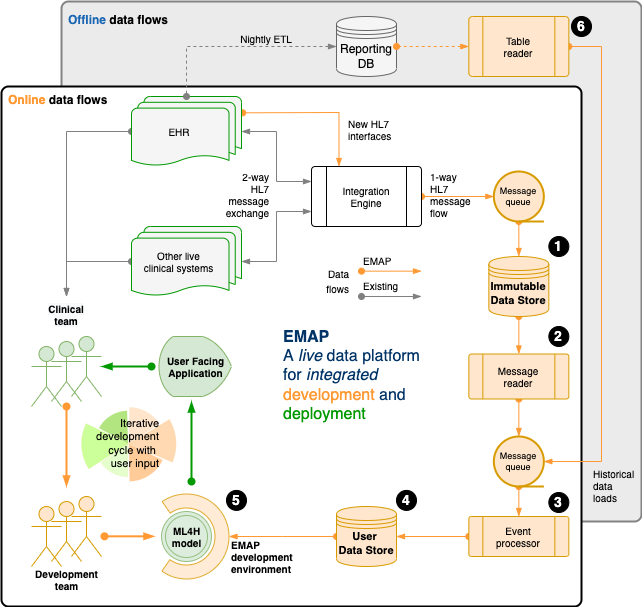
\includegraphics[width=10cm]{assets/emap.png}% This is a *.eps file
\end{center}
\caption{Our real-world development is performed on the  Experimental Medicine Application Platform (EMAP). EMAP is a clinical laboratory within which ML4H researchers can iteratively build, test and gather feedback from the bedside. It unifies the data and the tools for off-line and online development of ML4H models (see Figure 1 and the \textbf{(numbers)} in the following sentences that refer to objects in the figure).\newline
In brief, EMAP builds a patient orientated SQL database from Health Level 7 version 2 (HL7v2) messages that are being exchanged between hospital systems. HL7v2 messages are ubiquitous in health care, and the \textit{de facto} standard for internal communication. Rather than multiple pairwise connections between different hospital electronic systems, an integration engine acts as a single hub that routes HL7 messages, and where necessary translates to ensure compatibility. EMAP copies each message passing through the integration engine to a PostgreSQL database, the \textit{Immutable Data Store (IDS)} \textbf{(1)}. A \textit{message reader} \textbf{(2)} processes each live message to an interchange format so that downstream processing is insulated from local HL7 implementation. Separately, the \textit{table reader} \textbf{(6)} processes historical data (e.g. from the reporting database) to the same interchange format. Live messages take priority over historical messages in a queue that feeds the \textit{event processor} \textbf{(3)}. This links each message to a patient and a hospital visit, makes appropriate updates for out of order messages, and merges when separate identifiers are recognised to represent the same patient. A full audit trail is maintained. Each event updates a second live PostgreSQL database, the \textit{User Data Store} (UDS) \textbf{(4)}. The hospital hosts Jupyter and RStudio servers, and a Linux development environment is provided that allows docker deployment, installation of analysis libraries and frameworks, exposes SSH and HTTPS services, and allows user verification against the hospital active directory. \textbf{(5)} A typical workflow might include investigation and experimentation in a Jupyter Notebook with data from the UDS, then using a small network of docker containers to run the development script, log outputs to a testing database, and report to users via email or a locally hosted web application or dashboard.  A fuller explanation is available in the Electronic Supplementary Material (Section 2: EMAP data flows).}\label{fig:1}
\end{figure}


\begin{figure}[h!]
\begin{center}
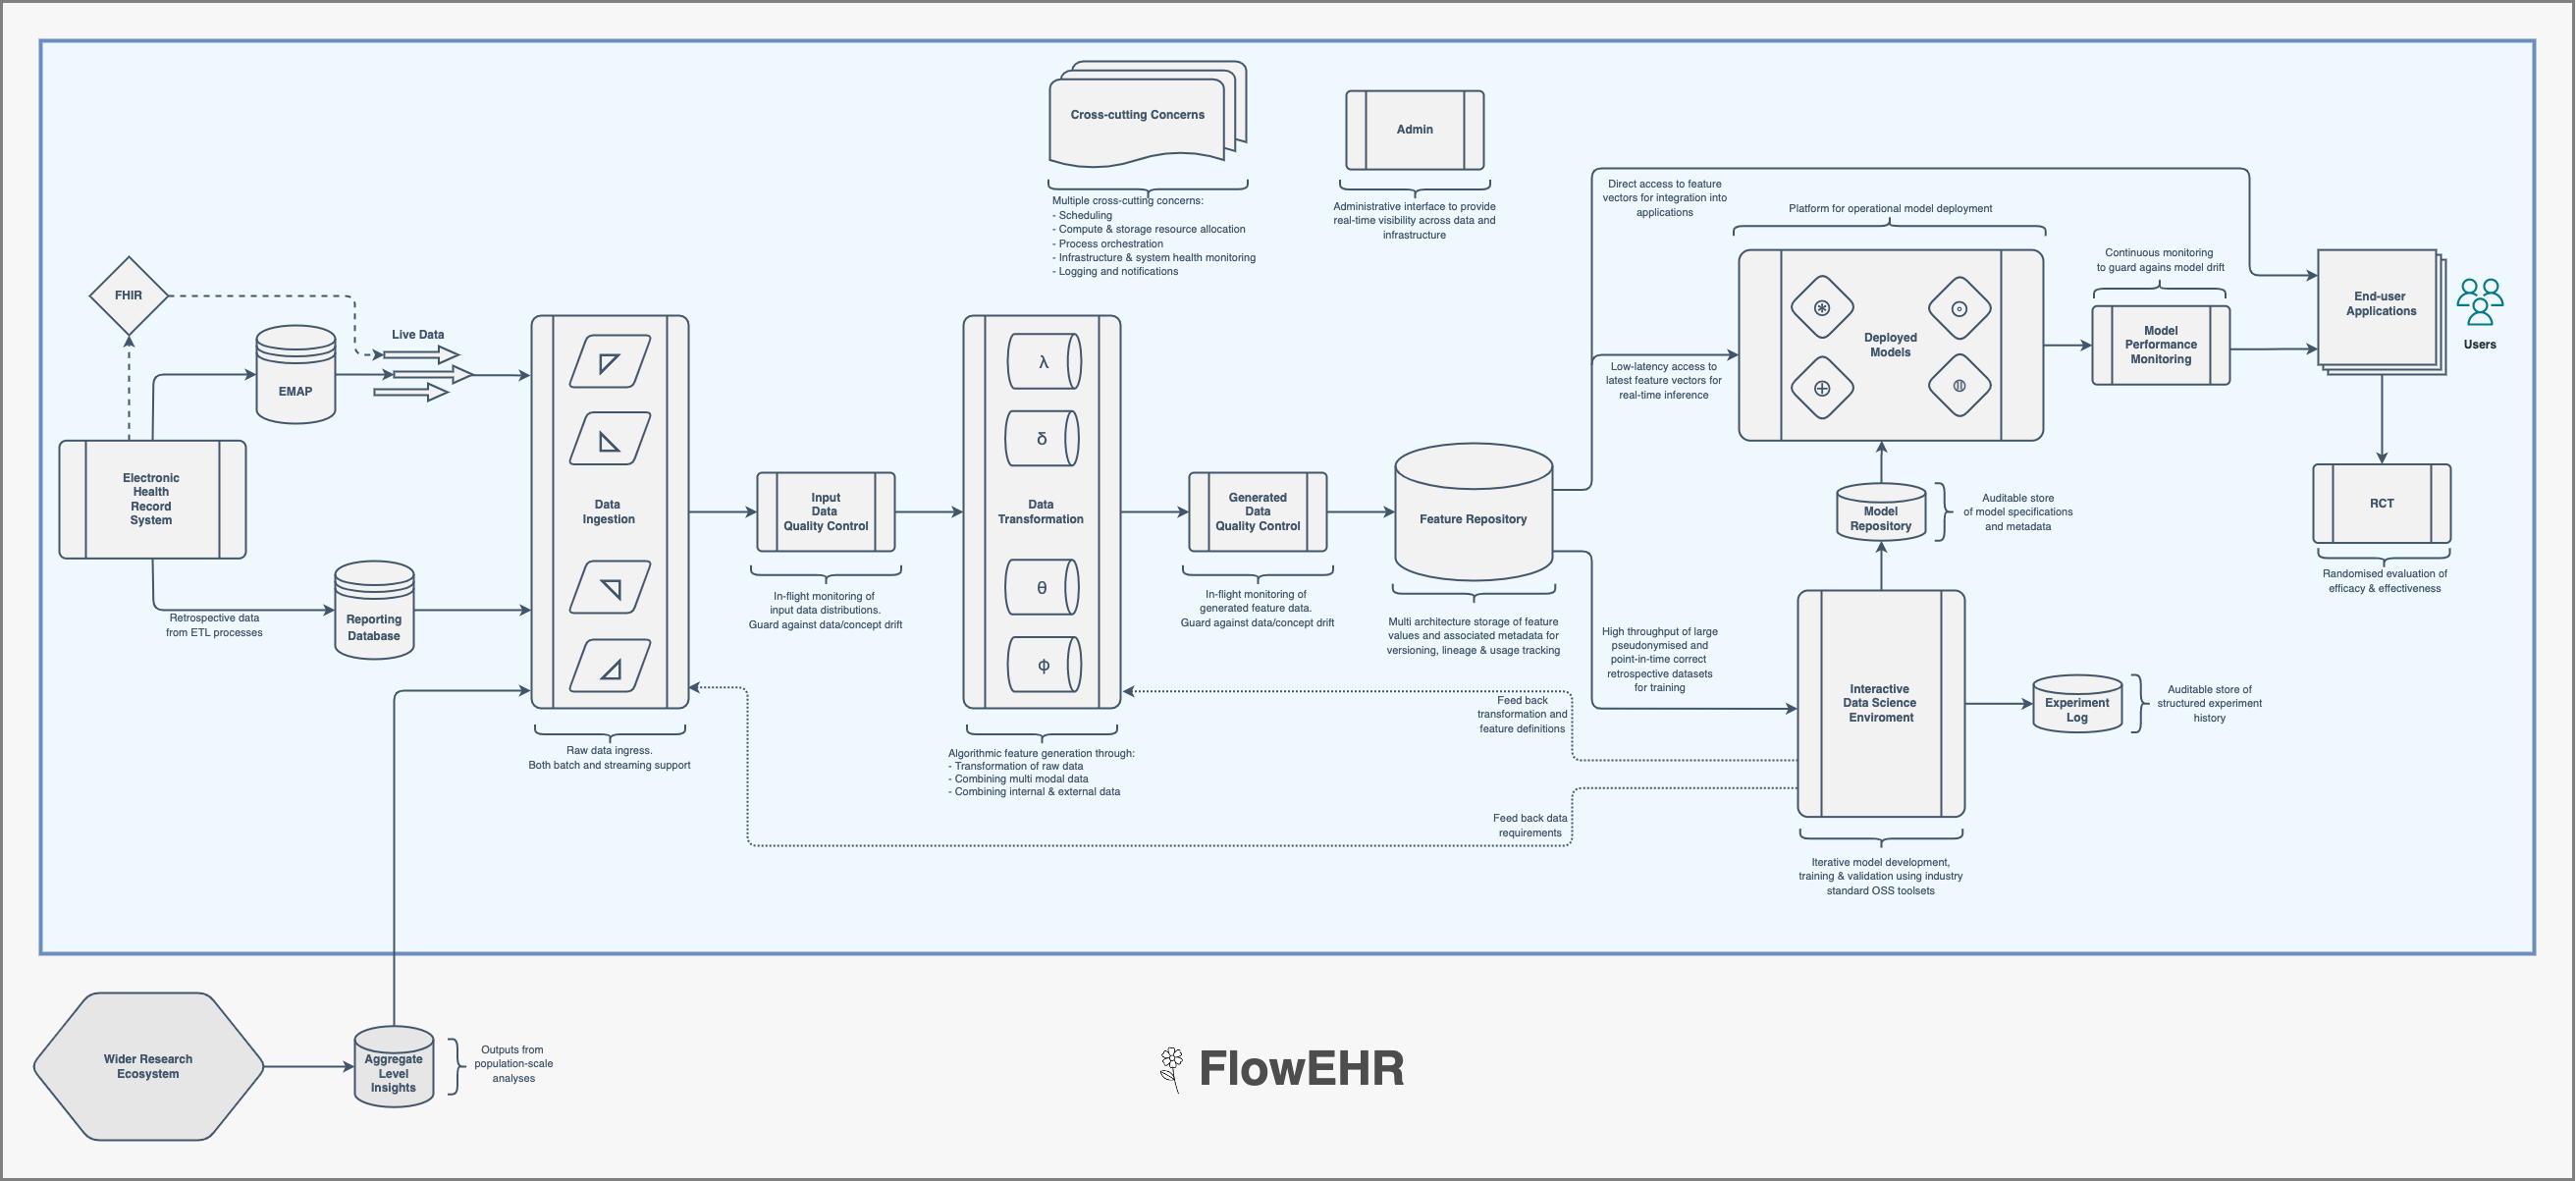
\includegraphics[width=15cm]{assets/flowehr.png}
\end{center}
\caption{
Our ML-Ops platform is called FlowEHR. Moving from left to right across the figure, the system monitors raw input data including checks for distribution shift, builds features with testable and quality controlled code, makes those features available to for both training and predictions to avoid train/serve skew, and maintains an auditable and monitored model repository.}\label{fig:2}
\end{figure}

%%% If you are submitting a figure with subfigures please combine these into one image file with part labels integrated.
%%% If you don't add the figures in the LaTeX files, please upload them when submitting the article.
%%% Frontiers will add the figures at the end of the provisional pdf automatically
%%% The use of LaTeX coding to draw Diagrams/Figures/Structures should be avoided. They should be external callouts including graphics.



\end{document}
